% -*- mode: noweb; noweb-default-code-mode: R-mode; -*-
\documentclass{beamer}
\usepackage{graphicx}
\usepackage{hyperref}
\usepackage[all]{xy}

\title{Sustainable R package development using documentation
  generation\\ \url{http://inlinedocs.r-forge.r-project.org}}
\author{Toby Dylan Hocking \\ toby.hocking AT inria.fr} \date{9 June
  2011}

\AtBeginSection[]
{
  \begin{frame}<beamer>
    \frametitle{Outline}
    \tableofcontents[currentsection]
  \end{frame}
}

\AtBeginSubsection[]
{
  \begin{frame}<beamer>
    \frametitle{Outline}
    \tableofcontents[currentsection,currentsubsection]
  \end{frame}
}
\newcommand{\framet}[2]{\frame[containsverbatim]{
\begin{itemize}
\frametitle{#1}{#2}
\end{itemize}
}}

\begin{document}
\setkeys{Gin}{width=\textwidth}
\frame{\titlepage}

\section{General package structure}

\framet{Sharing your code with the R community}{
\item Most likely you have some interesting functions you would like
  to share.
\item You could just email your code.R file to a colleague.
\item However, there is a standardized process for documenting,
  publishing and installing R code.
\item If you want your code to be used and modified by the R
  community, then you should consider making a \textbf{package}.
}

\framet{What is an R package?}{
\item It is a collection of code and data for a specific task, in a
  specific format.
\item Give your package a name, make a corresponding directory
  \texttt{pkgdir}
\item Required items:
  \begin{enumerate}
  \item \texttt{pkgdir/R/*.R} for R code.
  \item \texttt{pkgdir/DESCRIPTION} to describe its purpose, author,
    dependencies, etc.
  \item \texttt{pkgdir/man/*.Rd} for \textbf{documentation}.
  \end{enumerate}
\item Optional items:
  \begin{itemize}
  \item \texttt{pkgdir/data/*} for data sets.
  \item \texttt{pkgdir/src/*} for C/FORTRAN/C++ source to be compiled
    and linked to R.
  \item \texttt{pkgdir/inst/*} for other files you want to install.
  \item \texttt{pkgdir/po/*} for international translations.
  \end{itemize}
\item All of these need to be in a standard format as described in
  ``Writing R Extensions'' in excrutiating detail.
}

\framet{Why make an R package?}{
\item It seems pretty complicated to make a package, but in fact it is
  simple and comes with many benefits.
\item Advantages for you:
  \begin{enumerate}
  \item Installation from any internet-connected computer using
    \texttt{install.packages()} from the R command line. This includes
    \textbf{dependencies}!
  \item Compilation of C/C++/Fortran code on the CRAN servers, so
    Windows/Mac users can install your package even if they do not
    have a compiler.
  \end{enumerate}
\item Advantages for the R community:
  \begin{enumerate}
  \item Your package will be stored on CRAN, so others can make
    packages that depend on yours.
  \item Your code becomes open-source, so others can modify your code.
  \end{enumerate}
}

\framet{How to write the package?}{
\item Do it yourself! Read ``Writing R Extensions,'' only 163 pages in
  PDF form, as of R 2.13.0, 13 May 2011.\\
\item Luckily, there are several functions that use
  \textbf{documentation generation} to simplify the package-writing
  process.
\item \texttt{package.skeleton()}
\item \texttt{roxygen::roxygenize()}
\item \texttt{R.oo::Rdoc\$compile()}
\item \texttt{inlinedocs::package.skeleton.dx()}
}

\begin{frame} \frametitle{R source files and DESCRIPTION metadata are
    used to construct documentation Rd files}
  \def \objectstyle {\hbox}
  \xymatrix{
    \texttt{R/*.R} \ar@(d,l) [dr]  & \texttt{DESCRIPTION} \ar [d] & 
    \texttt{man/*.Rd}& \\
     & \txt{documentation\\generator} \ar@(r,d) [ur]& &\\
     &&package directory&\\
     \save "1,1"."3,4"*[F]\frm{}\restore
    }
\end{frame} 

\section{Documenting a function in several ways}

\begin{frame}\frametitle{Example: soft-thresholding function}
  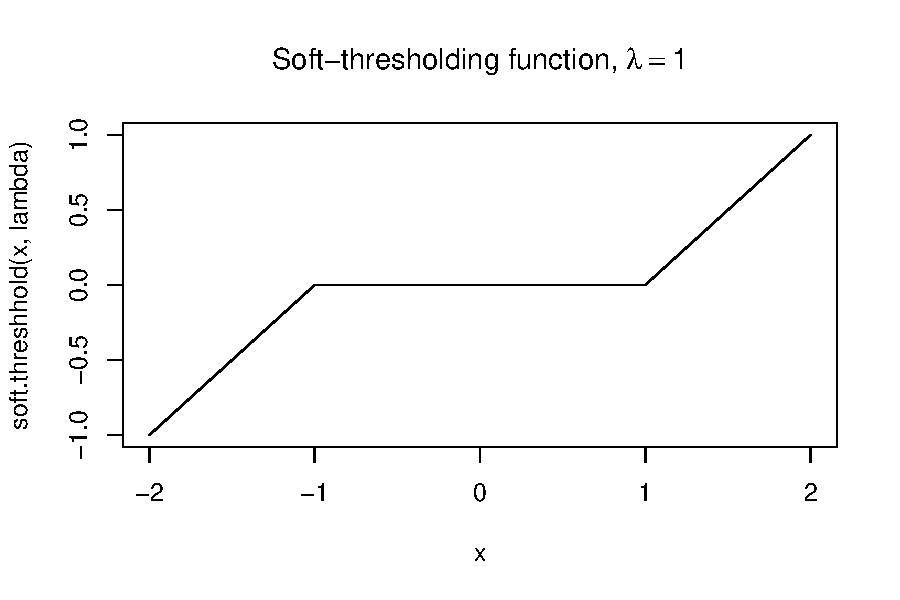
\includegraphics[width=\textwidth]{soft-thresh}
  $$f(x,\lambda)=\begin{cases}
    0 & |x|<\lambda\\
    x-\lambda\operatorname{sign}(x) & \text{otherwise}
  \end{cases}$$
\end{frame}

\begin{frame}[containsverbatim]
  \frametitle{R implementation of soft-thresholding function}
    $$f(x,\lambda)=\begin{cases}
    0 & |x|<\lambda\\
    x-\lambda\operatorname{sign}(x) & \text{otherwise}
  \end{cases}$$
  Make a new directory \texttt{softThresh} for the package,
  and put R code files in the \texttt{R} subdirectory:\\
    \texttt{softThresh/R/soft.threshold.R}
    \hrulefill
  \begin{verbatim}
  soft.threshold <- function(x,lambda=1){
    stopifnot(lambda>=0)
    ifelse(abs(x)<lambda,0,x-lambda*sign(x))
  }
  \end{verbatim}
\end{frame}

\subsection{Filling in \texttt{package.skeleton} templates by hand}

\begin{frame}[containsverbatim]
  \frametitle{Use \texttt{package.skeleton} to start a new package}
\begin{verbatim}
R> package.skeleton("softThresh",
                    code_files="soft.threshold.R")
\end{verbatim}
  will create \texttt{./softThresh/man|R|DESCRIPTION} with templates:
  \tiny
\begin{verbatim}
\name{soft.threshold}
\alias{soft.threshold}
%- Also NEED an '\alias' for EACH other topic documented here.
\title{
%%  ~~function to do ... ~~
}
\description{
%%  ~~ A concise (1-5 lines) description of what the function does. ~~
}
\usage{
soft.threshold(x, lambda = 1)
}
%- maybe also 'usage' for other objects documented here.
\arguments{
  \item{x}{
%%     ~~Describe \code{x} here~~
}
  \item{lambda}{
%%     ~~Describe \code{lambda} here~~
}
}
\details{
%%  ~~ If necessary, more details than the description above ~~
}
\value{
%%  ~Describe the value returned
%%  If it is a LIST, use
%%  \item{comp1 }{Description of 'comp1'}
%%  \item{comp2 }{Description of 'comp2'}
%% ...
}
\references{
%% ~put references to the literature/web site here ~
}
\author{
%%  ~~who you are~~
}
\note{
%%  ~~further notes~~
}

%% ~Make other sections like Warning with \section{Warning }{....} ~

\seealso{
%% ~~objects to See Also as \code{\link{help}}, ~~~
}
\examples{
##---- Should be DIRECTLY executable !! ----
##-- ==>  Define data, use random,
##--	or do  help(data=index)  for the standard data sets.

## The function is currently defined as
function (x, lambda = 1) 
{
    stopifnot(lambda >= 0)
    ifelse(abs(x) < lambda, 0, x - sign(x) * lambda)
  }
}
% Add one or more standard keywords, see file 'KEYWORDS' in the
% R documentation directory.
\keyword{ ~kwd1 }
\keyword{ ~kwd2 }% __ONLY ONE__ keyword per line
\end{verbatim}
\end{frame}

\begin{frame}[containsverbatim]
  \frametitle{Fill in the Rd templates generated by \texttt{package.skeleton}}
  \texttt{softThresh/man/soft.threshold.Rd}
  \hrulefill
  \scriptsize
\begin{verbatim}
\name{soft.threshold}
\title{Soft-thresholding}
\description{Apply the soft-threshold function to a vector.}
\usage{
soft.threshold(x, lambda = 1)
}
\arguments{
  \item{x}{A vector of numeric data.}
  \item{lambda}{The largest absolute 
    value that will be mapped to zero.}
}
\value{The vector of observations
    after applying the soft-thresholding.}
\author{Toby Dylan Hocking <toby.hocking@inria.fr>}
\examples{
  x <- seq(-5,5,l=50)
  y <- soft.threshold(x)
  plot(x,y)
}
\end{verbatim}
\end{frame}

\begin{frame}[containsverbatim]
  \frametitle{Write the metadata in the DESCRIPTION file}
  \texttt{softThresh/DESCRIPTION}
  \hrulefill
  \begin{verbatim}
  Package: softThresh
  Maintainer: Toby Dylan Hocking <toby.hocking@inria.fr>
  Author: Toby Dylan Hocking
  Version: 1.0
  License: GPL-3
  Title: Soft-thresholding
  Description: A package documented by hand.
\end{verbatim}
\end{frame}

\framet{Doing it by hand versus documentation generation}{
  \item Doing it by hand is simple but has some disadvantages
    \begin{itemize}
    \item Easy to do, \LaTeX-like syntax
    \item Possibility of conflict between code and documentation
    \item Every time the function changes, need to copy to docs
    \end{itemize}
  \item Documentation generation has several advantages
    \begin{itemize}
\item Documentation is written in comments, nearer to the source code
\item Can exploit the structure of the source code
\item Simplifies updating documentation (!!)
\item Reduces the probability of mismatch between code and docs
  \end{itemize}
}

\framet{Different approaches to documentation generation}{
\item Put the documentation in a big header comment
  \begin{itemize}
    \item roxygen::roxygenize()
    \item R.oo::Rdoc\$compile()
  \end{itemize}
\item Put the documentation in comments right next to the relevant code
  \begin{itemize}
  \item inlinedocs::package.skeleton.dx()
  \end{itemize}
}

\subsection{Doc generation from headers using roxygen and R.oo::Rdoc}

\begin{frame}[containsverbatim]
  \frametitle{roxygen reads documentation from comments above}
  \texttt{softThresh/R/soft.threshold.R}
  \hrulefill
\begin{verbatim}
##' Apply the soft-threshold function to a vector.
##' 
##' @title Soft-thresholding
##' @param x A vector of numeric data.
##' @param lambda The largest absolute value that
##' will be mapped to zero.
##' @return The vector of observations after applying the
##' soft-thresholding.
##' @author Toby Dylan Hocking <toby.hocking@@inria.fr>
soft.threshhold <- function(x,lambda=1){
  stopifnot(lambda>=0)
  ifelse(abs(x)<lambda,0,x-sign(x)*lambda)
}
\end{verbatim}
  Note: headers can be automatically generated using the
  \texttt{ess-roxy-update-entry C-c C-o} command in Emacs+ESS.
\end{frame}

\begin{frame}[containsverbatim]
  \frametitle{roxygen generates Rd}
  \texttt{shell\$ R CMD roxygen -d softThresh}
  \\
  generates/overwrites \texttt{softThresh/man/soft.threshold.Rd}
  \\ \hrulefill\\
  There is also the R function \texttt{roxygenize} (see its help page for
  details)
\end{frame}

\begin{frame}
  \frametitle{roxygen can also generate call graphs (complicated setup)}
  {\scriptsize Source: \url{http://r-forge.r-project.org/scm/viewvc.php/*checkout*/pkg/inst/doc/Compose-callgraph.pdf?root=roxygen}}
  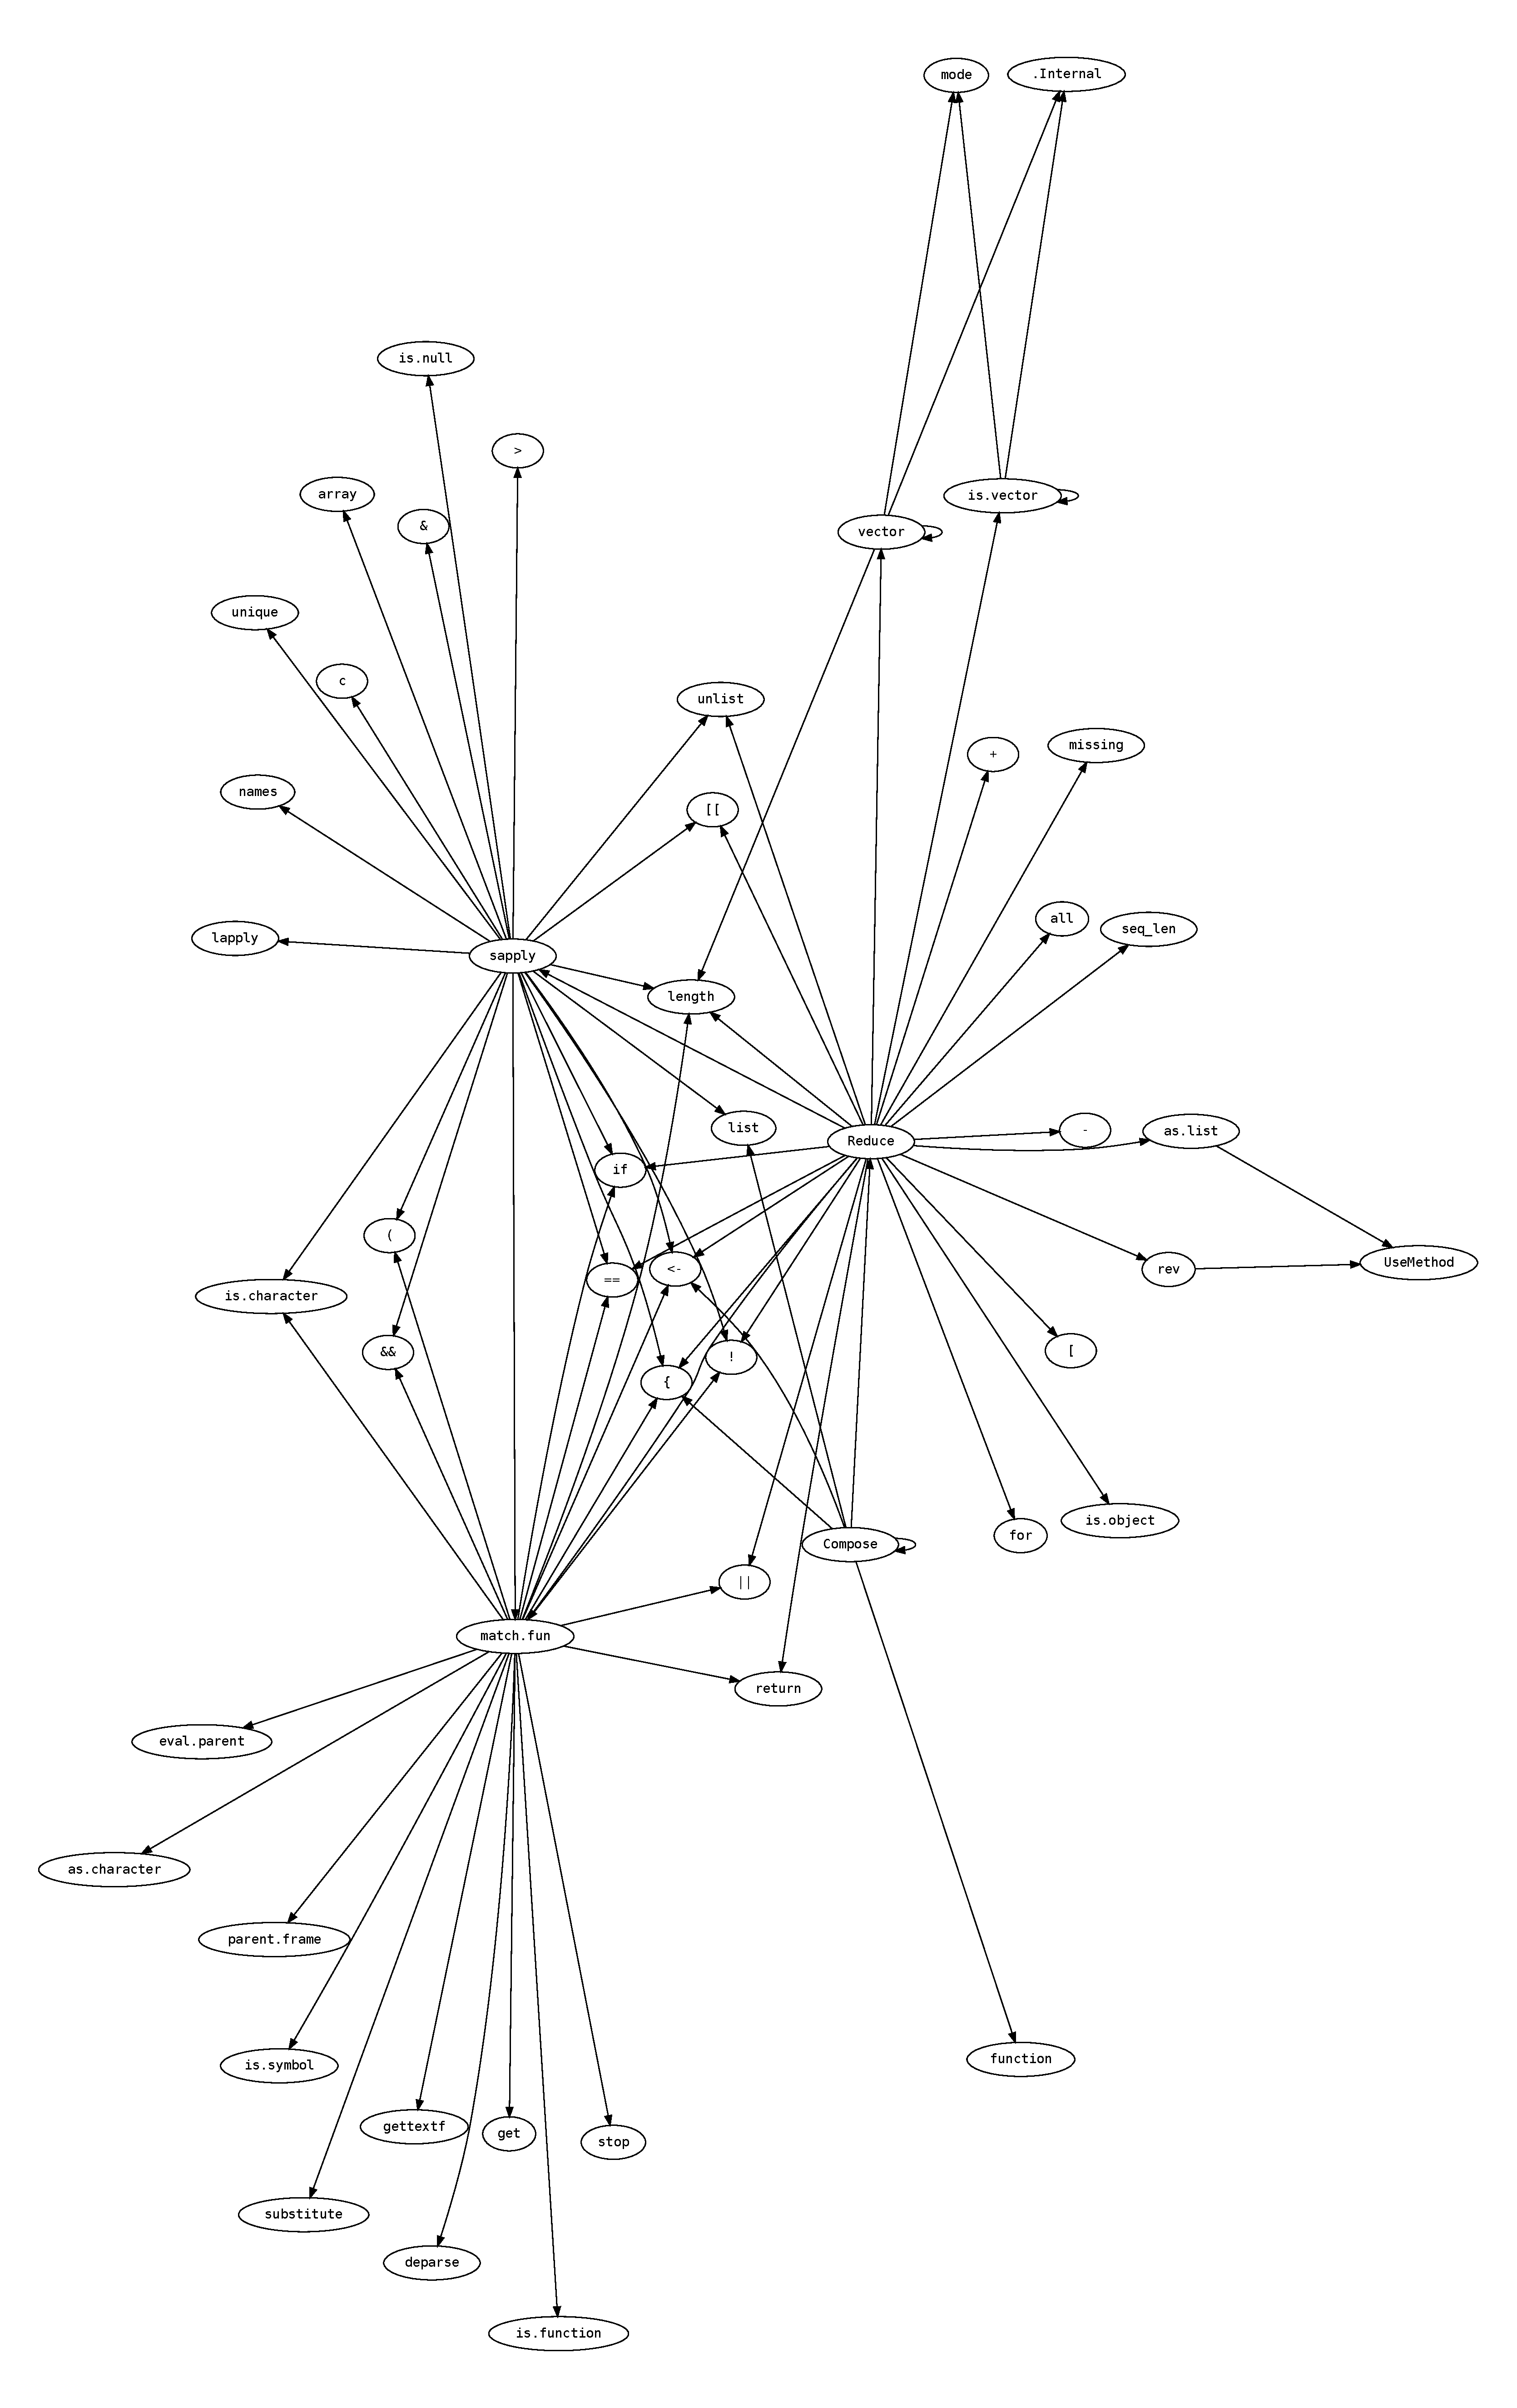
\includegraphics{Compose-callgraph}
\end{frame}

\begin{frame}[containsverbatim]
  \frametitle{Rdoc puts docs in headers as well}
  (similar to roxygen, but less documentation and editor support)
  \small
\begin{verbatim}
## @RdocFunction soft.threshold
## @title "Soft-thresholding"
## \description{
##  Apply the soft-threshold function to a vector.
## }
## @synopsis
## \arguments{
##   \item{x}{A vector of numeric data.}
##   \item{lambda}{The largest absolute value 
##      that will be mapped to zero.}
## }
## \value{
## The vector of observations after applying the
## soft-thresholding.
## }
## @author
\end{verbatim}
\end{frame}

\framet{Documentation generation based on comments in headers}{
  \item 2 step process:
  \begin{enumerate}
\item Write: documentation written in comments.
\item Compile: comments automatically translated to Rd files.
  \end{enumerate}
\item Advantages:
  \begin{itemize}
  \item Documentation closer to code.
  \item Less chance of mismatch.
  \item Fewer manual documentation updates when the code changes.
  \end{itemize}
\item Disadvantages:
  \begin{itemize}
  \item Need to copy function argument names in the header.
  \item The header is sometimes really big.
  \item In reality, the docs are far away from the corresponding code.
  \end{itemize}
\item Can we come up with a system where the documentation is even
  closer to the actual code?
}
% \framet{Visualizing your functions using call graphs}{
% \item @callGraph
% }

\subsection{Doc generation from inline comments using inlinedocs} 

\begin{frame}[containsverbatim]
  \frametitle{inlinedocs allows docs in comments adjacent to the code}
  \texttt{softThresh/R/soft.threshold.R}
  \hrulefill
  \small
\begin{verbatim}
soft.threshold <- function # Soft-thresholding
### Apply the soft-threshold function to a vector.
(x,
### A vector of numeric data.
 lambda=1
### The largest absolute value that will be mapped to zero.
 ){
  stopifnot(lambda>=0)
  ifelse(abs(x)<lambda,0,x-sign(x)*lambda)
### The vector of observations after applying 
### the soft-thresholding function.
}
\end{verbatim}
\end{frame}

\begin{frame}[containsverbatim]
  \frametitle{another inlinedocs syntax for function arguments}
  \texttt{softThresh/R/soft.threshold.R}
  \hrulefill
  \small
\begin{verbatim}
soft.threshold <- function # Soft-thresholding
### Apply the soft-threshold function to a vector.
(x,       ##<< A vector of numeric data.
 lambda=1 ##<< The largest absolute value that
          ##   will be mapped to zero.
 ){
  stopifnot(lambda>=0)
  ifelse(abs(x)<lambda,0,x-sign(x)*lambda)
### The vector of observations after applying 
### the soft-thresholding function.
}
\end{verbatim}
\end{frame}

\begin{frame}[containsverbatim]
  \frametitle{inlinedocs: comment code wherever it is relevant}
  \texttt{softThresh/R/soft.threshold.R}
  \hrulefill
  \small
\begin{verbatim}
soft.threshold <- function # Soft-thresholding
### Apply the soft-threshold function to a vector.
(x,       ##<< A vector of numeric data.
 lambda=1 ##<< The largest absolute value that
          ##   will be mapped to zero.
 ){
  stopifnot(lambda>=0)
  ##details<< lambda must be non-negative.
  ifelse(abs(x)<lambda,0,x-sign(x)*lambda)
### The vector of observations after applying 
### the soft-thresholding function.
}
\end{verbatim}
\end{frame}

\begin{frame}[containsverbatim]
  \frametitle{inlinedocs::package.skeleton.dx() generates Rd files}
  \begin{verbatim}
R> library(inlinedocs)
R> package.skeleton.dx("softThresh")
\end{verbatim}
  produces \texttt{softThresh/man/soft.threshold.Rd}
\end{frame}

\begin{frame}[containsverbatim]
  \frametitle{How to write example code?}
    roxygen: in comments (not executable)
    \hrulefill
\begin{verbatim}
##' @examples
##' x <- seq(-5,5,l=50)
##' y <- soft.threshold(x)
##' plot(x,y)
soft.threshold <- function(x,lambda=1){...}
\end{verbatim}
    inlinedocs: in code (executable)
    \hrulefill
    \begin{verbatim}
soft.threshold <- structure(function(x,lambda=1){
  ...
},ex=function(){
  x <- seq(-5,5,l=50)
  y <- soft.threshold(x)
  plot(x,y)
})
\end{verbatim}
\end{frame}

\framet{inlinedocs for documentation generation}{
  \item 2 step write/compile process for documentation generation.
  \item Write the documentation in comments \textbf{right next to} the
    corresponding code.
  \item Takes advantage of function argument names, etc. defined in
    the code.
  \item Resulting code base is very easy to maintain.
  \item Almost eliminates the possibility of code and documentation
    conflicts.
  \item AND: support for S4 methods, named list documentation, easily
    extensible syntax.}
  
\section{Package publication, conclusions, and references}

\framet{To publish your package}{
  \item Write your code in \texttt{pkgdir/R/code.R}
  \item Write a \texttt{pkgdir/DESCRIPTION}
  \item Write (or generate) documentation \texttt{pkgdir/man/*.Rd}
  \item \texttt{R CMD check pkgdir} (until no errors or warnings)
  \item \texttt{R CMD build pkgdir} (makes \texttt{pkgdir.tar.gz})
  \item Upload \texttt{pkgdir.tar.gz} to ftp://cran.r-project.org/incoming 
    \begin{itemize}
    \item     user: anonymous
    \item password: your@email
      \item send email to cran@r-project.org
    \end{itemize}
  \item If it passes the CRAN checks, then it is posted to the CRAN
    website for anyone to download and install using \texttt{install.packages()}
  }

\framet{References for learning more about package development}{
\item The definitive guide: help.start() then
  \href{http://cran.r-project.org/doc/manuals/R-exts.html}{Writing R
    Extensions}
\item The built-in package generator: ?package.skeleton
\item roxygen
  \begin{itemize}
  \item library(roxygen)
  \item ?roxygenize
  \item \url{http://roxygen.org/roxygen.pdf}
  \end{itemize}
\item R.oo:Rdoc
  \begin{itemize}
  \item library(R.oo)
  \item ?Rdoc (not very much documentation)
  \item \url{http://www.aroma-project.org/developers}
  \end{itemize}
\item inlinedocs
  \begin{itemize}
  \item library(inlinedocs)
  \item ?inlinedocs
  \item \url{http://inlinedocs.r-forge.r-project.org}
  \end{itemize}
\item Contact me directly: toby.hocking AT inria.fr,
  \url{http://cbio.ensmp.fr/~thocking/}
}

\end{document}

